\subsection{Controlador}
El controlador en un MVC es el responsable de recibir y procesar la entrada del usuario y actualizar el modelo. En esta práctica, dicha responsabilidad es la de calcular la distancia de Levenshtein y transformar los resultados de dicho algoritmo a diferentes estructuras de datos.

\subsubsection{Diseño}
El controlador se separa en dos grandes secciones como ya se ha mencionado previamente. \\

Por una parte, calcular la distancia de Levenshtein entre dos conjuntos de idiomas. Usando \say{method overloading} \cite{Method Overloading}, podemos abstraer Levenshtein para que acepte dos palabras, dos idiomas o que gestione la comunicación y preparación de los datos para lanzar una de sus posibles variedades previamente estipuladas.\\

Por otra parte, y debido a la necesidad de representar los resultados de diferentes maneras en la vista, este se encarga de, una vez obtenida una solución de ejecutar Levenshtein, transformar dicha solución a las diferentes posibles estructuras necesarias. Específicamente, se encarga de convertir dicha solución en un  grafo de distancias y el árbol filogenético \cite{Phylogenetic tree}

\subsubsection{Levensthein}

La distancia de Levenshtein permite identificar la \say{distancia} entre dos cadenas de valores; véase, cuantas modificaciones tendríamos que hacer en uno para que sea el segundo. Estas modificaciones son, para una posición \textit{i}:\\

\begin{itemize}
    \item Cambiar su valor
    \item Eliminarlo
    \item Añadir un valor
\end{itemize}\bigskip

Es extremadamente popular para verificar la ortografía de un texto, analizar secuencias de ADN, \say{data mining} y procesamiento del lenguaje natural; entre otros. Con respecto a su implementación, y aunque existen otros acercamientos, se ha decidido aplicar el concepto de programación dinámica para \say{cachear} valores previamente ya calculados. De esta manera, evitamos repetir cálculos y aceleramos su proceso pagando un coste adicional en memoria. Una posible implementación de la distancia de Levenshtein con programación dinámica podría ser el siguiente:

\begin{code}{\scriptsize}{pascal}
function LevenshteinDistance(char s[1..m], char t[1..n]):
  // for all i and j, d[i,j] will hold the Levenshtein distance between
  // the first i characters of s and the first j characters of t
  declare int d[0..m, 0..n]
 
  set each element in d to zero
 
  // source prefixes can be transformed into empty string by
  // dropping all characters
  for i from 1 to m:
    d[i, 0] := i
 
  // target prefixes can be reached from empty source prefix
  // by inserting every character
  for j from 1 to n:
    d[0, j] := j
 
  for j from 1 to n:
    for i from 1 to m:
      if s[i] = t[j]:
        substitutionCost := 0
      else:
        substitutionCost := 1

      d[i, j] := minimum(d[i-1, j] + 1,                   
                         d[i, j-1] + 1,                   
                         d[i-1, j-1] + substitutionCost)  
 
  return d[m, n]
\end{code}

Con respecto a la complejidad temporal, podemos asegurar que, para una palabra con otra, es $O(src * dst)$ donde \textit{src} y \textit{dst} son las longitudes de las cadenas de entrada; ya que creamos dos bucles anidados cuyo límite es \textit{src} y \textit{dst}. El algoritmo, como ya se ha citado previamente, se ha implementado aplicando programación dinámica, por lo que crea una matriz de tamaño $(src + 1) \times (dst + 1)$ y rellenándola iterativamente. Dado que el cálculo de una celda es tiempo constante, la complejidad temporal general del algoritmo dependerá del tamaño de la matriz y como esta tiene como parámetros \textit{src} y \textit{dst}, reafirmamos que la complejidad temporal es de $O(src * dst)$ \\

Con respecto al coste espacial, debido a que tenemos que generar una matriz de datos proporcional al tamaño de las cadenas de entrada, obtenemos $O(src * dst)$.

\paragraph{Estudios}
Debido a la gran cantidad de datos usados para este proyecto, la aplicación ofrece una opción para ejecutar los cálculos paralelamente, al no depender los resultados de los previos. Sin embargo, debido al sistema de \textit{Notify Request}, la aplicación es nativamente paralela y usará tantos procesos como la CPU del hardware pueda lanzar. Debido al interés académico, se implementó una estructura que permite lanzar el algoritmo de manera secuencial:

\begin{figure}[!h]
    \centering
    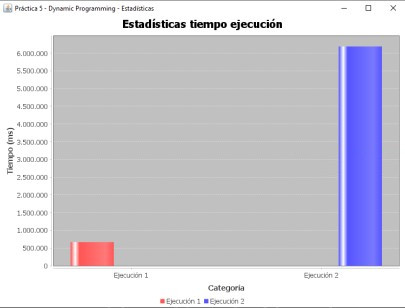
\includegraphics[width=\linewidth]{MVC/Controller/img/stats.jpg}
    \caption{Estadísticas temporales en milisegundos}
    \label{fig:time_stats}
\end{figure}\bigskip

Como se puede apreciar, a la izquierda se postra la ejecución paralela y a la derecha la secuencial. Ambas compararon todos los diccionarios entre ellos con diez mil palabras de resolución. Esto es, cada vez que se aplicó Levenshtein se cogieron diez mil palabras aleatorias del lenguaje. Bajo este benchmark sacamos los siguientes datos:\\

\begin{multicols}{2}

\textbf{Paralela}
\begin{itemize}
    \item \textbf{CPU}: 100\% 
    \item \textbf{Tiempo}: 10 min
\end{itemize}
\vfill
\null
\columnbreak

\textbf{Secuencial}
\begin{itemize}
    \item \textbf{CPU}: 12\% 
    \item \textbf{Tiempo}: 103 min 
\end{itemize}
\vfill
\null
\end{multicols}

Podemos observar que, aunque la ejecución paralela tarda aproximadamente diez veces más, también consume diez veces más los recursos del \say{hardware}. Esto nos indica que, al menos para la máquina en la que se ha ejecutado el benchmark, podemos usar ambas ejecuciones según nuestras prioridades.

\subsubsection{Transformación de estructuras de datos}
Ya que nuestra aplicación permite la visualización de los pesos de Levenshtein tanto en grafo como en un árbol filogenético\cite{Phylogenetic tree}, es necesario transformar los datos devueltos por este a dichas estructuras. Técnicamente, el algoritmo de Levenshtein dados un conjunto de lenguajes devuelve un \say{hashmap} cuyos claves son las parejas de lenguajes y los valores son los pesos. Para ello se han creado dos estructuras de datos que permiten representar dichas estructuras.\\

Para el grafo, creamos un conjunto cuyos valores son los diferentes idiomas en los que se ha ejecutado la distancia de Levenshtein. Iteramos bajo él y creamos todas las posibles conexiones con los demás lenguajes y obtenemos el peso accediendo al \say{hashmap}. Finalmente, devolvemos un array con todos los lenguajes, sus conexiones y sus pesos.\\

Para el árbol podemos usar el grafo previamente mencionado, ya que podemos saber para un lenguaje cuáles son los pesos y por ende, podemos ordenarlos de menor a mayor. Usamos el algoritmo de Kruskal\cite{Kruskal algorithm} para obtener el árbol mínimo dado un grafo no dirigido ponderado por aristas cuyo pseudocódigo podría ser tal que:

\begin{code}{\scriptsize}{python}
algorithm Kruskal(G) is
    F:= @$\O$@
    for each v @$\in$@ G.V do
        MAKE-SET(v)
    for each (u, v) in G.E ordered by weight(u, v), increasing do
        if FIND-SET(u) @$\neq$@ FIND-SET(v) then
            F:= F @$\cup$@ {(u, v)} @$\cup$@ {(v, u)}
            UNION(FIND-SET(u), FIND-SET(v))
    return F
\end{code}

\subsubsection{Adivinador de palabras}\label{Word Guesser expl}

Para el adivinador de palabras, se emplean dos estrategias:\bigskip

La primera es una versión modificada de nuestra estructura de Levenshtein. Creamos un diccionario \say{custom} cuyas palabras son las escritas por el usuario por input, y ejecutamos Levenshtein con todos los lenguajes con una resolución de dos mil palabras. El resultado, como ya explicado previamente, es un \say{hashmap} cuyos valores representan las distancias. Usando una simple fórmula para mapear todas las distancias a una probabilidad: 
\[probabilidad = \frac{1}{distancia + 1}\]
Podemos mostrar todas las probabilidades y escoger aquella que sea mayor.\bigskip

La segunda, es un modelo generativo conocido como clasificador de Naive Bayes, este se basa en que las características de las palabras son independientes, es decir, supone que las probabilidades de característica $p(x_j|y)$ son independientes $p(x|y = c) = \prod_{j=1}^n p(x_j|y = c)$ dada la clase c. Este, se basa en la función de regresión lineal 

\[\theta_{j|y=c} = p(x_j|y = c) = \frac{count(x_i,y = c) + 1}{\sum_{i=1}^m count(x_i,y = c) + |V|}\]

donde, finalmente se le aplicará una función de softmax para obtener las probabilidades normalizadas, por lo que, quedaría de la siguiente forma: 

\[\text{softmax}(x_i) = \log\left(\frac{e^{x_i}}{\sum_{j=1}^{n} e^{x_j}}\right)\]
